%%----------------------------------------------------------------------
%%----------------------------------------------------------------------
\clearpage
\pagetitle{Introduction}

\begin{columns}

  \emph{Legacies} is an unofficial, team-oriented skirmish campaign
  for Games Workshop's \emph{Warhammer 40,000}.  Its core is a set of
  eight thematic missions designed for \emph{Recon Squad}, an
  unofficial skirmish variant of \emph{40k} similar to Games
  Workshop's \emph{Kill Team} rules.  In a Recon Squad game, players
  field only a squad or two on a small board with dense terrain, and
  all of their models act independently.  This makes for a very
  different \emph{40k} experience, focused on the heroics and
  sacrificies of everyday grunts and squad leaders, while still using
  the standard gameplay rules you already know and the models you
  love.

  Those skirmish missions are woven into a campaign by a set of eight
  Legacies, specific missions the recon squads are striving to
  complete for their alliance.  The climax of the campaign is the
  Cataclysm, in which all the recon squads and some reinforcements
  fight alongside their alliance teammates in a final joint battle
  while also trying to fulfill their legacy.

  \emph{Legacies} is may be run either as a single full-day event or
  over several evenings.  Though the missions and legacies are
  thematic and storyful, \emph{Legacies} does not have its own
  setting, so that it can be easily adapted to one of your own making.
  Other events are also easily connected before or after this campaign
  to form a larger narrative.  Notes are also included here on scoring
  \emph{Legacies} in a narrative tournament or league, with individual
  prizes.

\missionheading{Overview}

\emph{Legacies} is played as four rounds of Recon Squad skirmishes,
each capturing a small but pivotal incident in a larger battle,
followed by a closing Cataclysm team battle.  Rules for Recon Squad
are here:

\bigskip%
\centerline{\url{http://rocketshipgames.com/40k/recon-squad/}}

\bigskip%
Each recon squad is working toward a particular legacy inside the
grand history of the greater conflict:

\begin{squishitemize}
\item \textbf{Bodyguards:} Fierce defenders of critical battlefield
  leaders and personnel;

\item \textbf{Excavators:} Daring explorers, technical experts, and
  artifact raiders \emph{par excellence};

\item \textbf{Headhunters:} Precision instruments of assassination and
  targeted violence;
\end{squishitemize}

  % Following the events of \emph{The Debacle on Caldor IV} it has
  % become clear that the legendary \emph{Scythe of Unbound Light}
  % exists and is immeasurably important.  This discovery has spun the
  % maelstrom of conflict on Caldor IV to even dizzier velocities.
  % Unfortunately, the destruction of the planet is also now inevitable
  % with the Imperium having begun Exterminatus.  With every army
  % shattered and communication all but impossible, it is up to the
  % individual commanders and warriors in the field to rise to the
  % moment.  \emph{The Twilight of Caldor IV} plots the heroics of small
  % bands of warriors furiously moving into position to help their
  % alliance claim the relic before the end.

%\columnbreak
\noindent\fbox{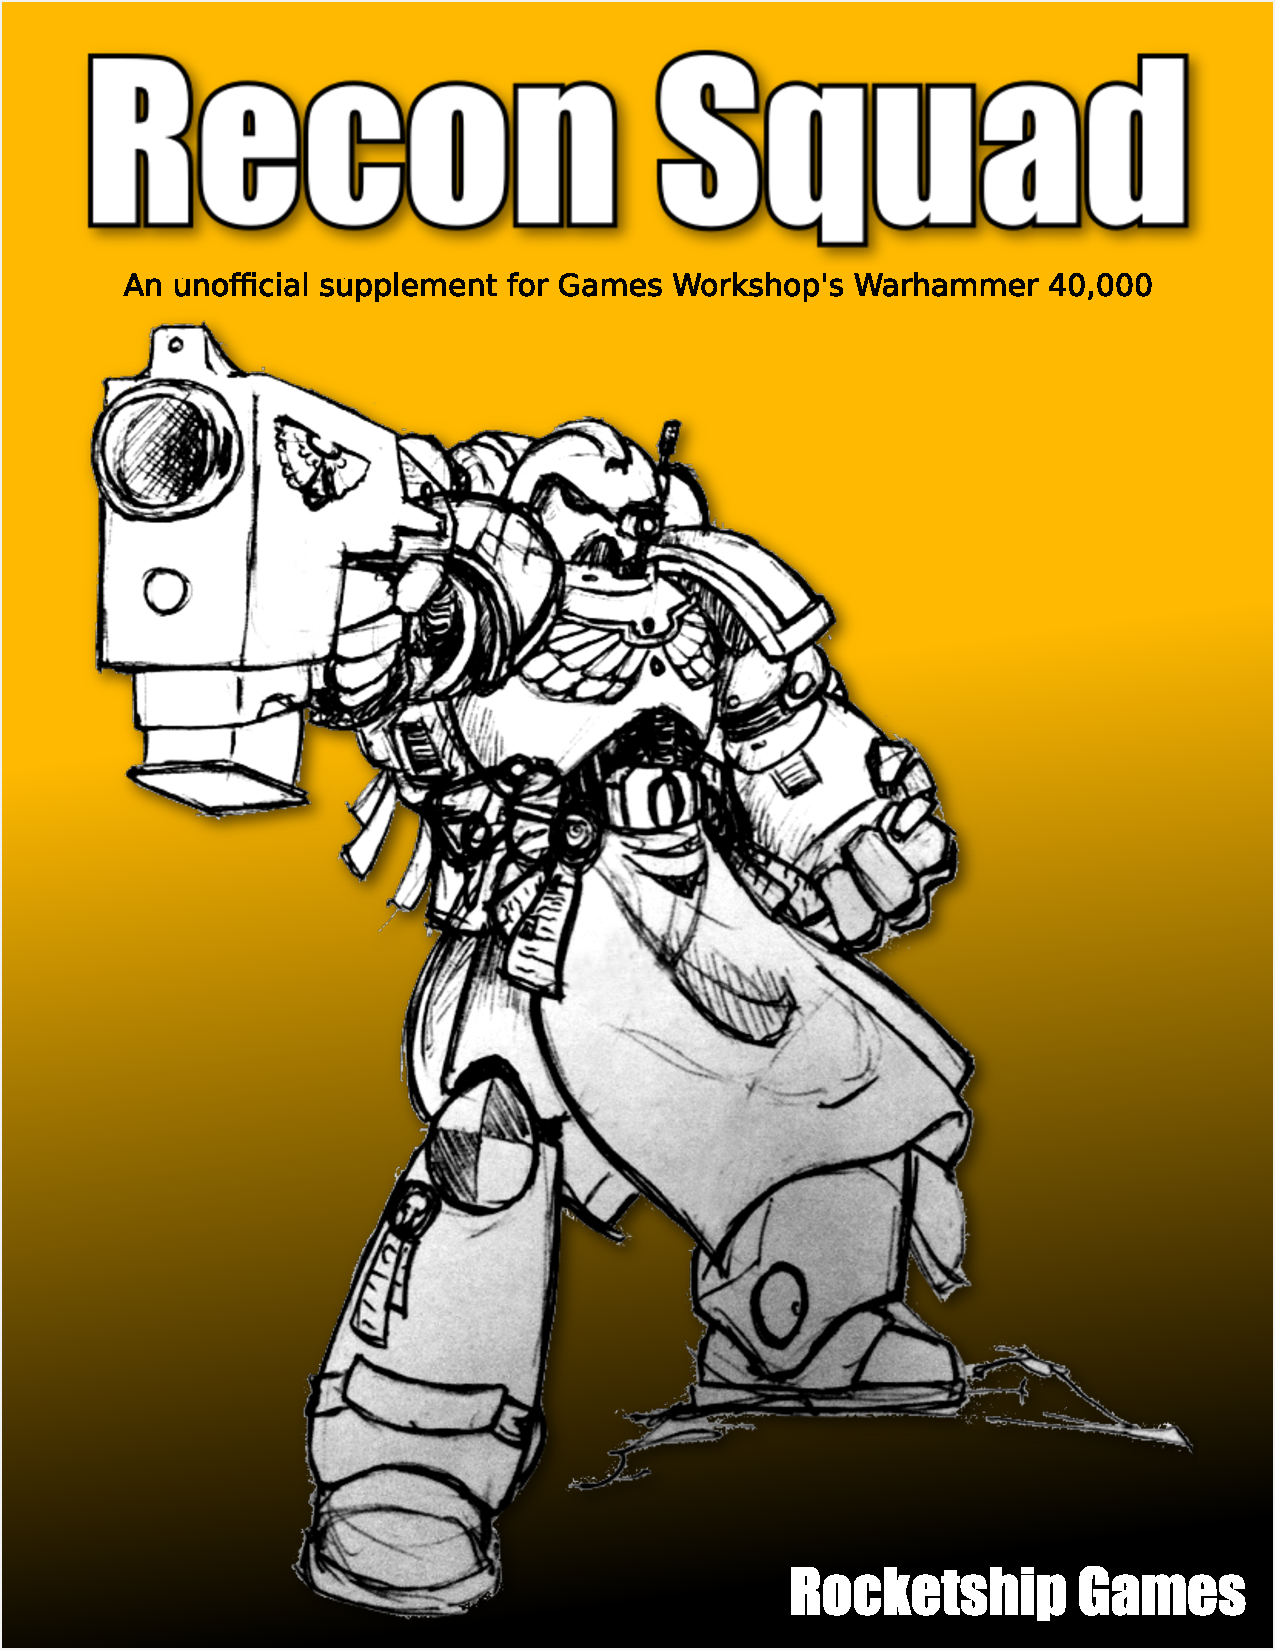
\includegraphics[width=\linewidth]{art/recon-squad.pdf}}

\begin{squishitemize}
\item \textbf{Killers:} Shattered fighters disconnected from anything
  but maniacal bloodshed;

\item \textbf{Penetrators:} Sharpened blades able to break through any
  armor or defense;

\item \textbf{Scouts:} Reckless adventurers dancing in the jaws of
  death for more information;

\item \textbf{Sentinels:} Implacable defenders and masters of
  impromptu fortification building;

\item \textbf{Warriors:} Hardened veterans that have been through
  everything and haven't seen the end.
\end{squishitemize}

Their path toward those legacies is defined by the missions they
tackle, as attackers or defenders:

\smallskip\centerline{\begin{tabular}{C{1.25in}C{1.25in}}
\textbf{Ambush} & \textbf{Encirclement}\\
\textbf{Assassination} & \textbf{Excavation}\\
\textbf{Battlefield} & \textbf{Installation}\\
\textbf{Breakthrough} & \textbf{Skirmish}\\
\end{tabular}}

\smallskip%
Successes and failures at those challenges will define both the recon
squad's place in history, and their alliance's ability to win the
Cataclysm.

\end{columns}
